% Revised Vision Research manuscript; all numerical results refer to the audited study.
\documentclass[authoryear,preprint,review,12pt]{elsarticle}
\usepackage{amsmath,amssymb,booktabs,graphicx,tabularx,longtable}
\usepackage{lineno}
\usepackage{microtype}
\setlength{\emergencystretch}{2em}
\usepackage[hidelinks,hypertexnames=false]{hyperref}
\usepackage{url}
\journal{Vision Research}
\begin{document}
\begingroup
\renewcommand{\baselinestretch}{1}\selectfont
\begin{frontmatter}
\title{Task, spatial support, and reference cues shape learned color representations}
\author[inst1]{Mohammad Rostami\corref{cor1}}
\ead{mrostami@seas.upenn.edu}
\cortext[cor1]{Corresponding author}
\affiliation[inst1]{organization={Amazon Generative AI Innovation Center},country={USA}}
\fntext[fn1]{This work is independent from the author's position at Amazon.}
\begin{abstract}
Task-trained networks can reveal which aspects of color coding depend on behavioral objectives and model constraints. We compare reflectance-category classification and illuminant-temperature estimation using small convolutional networks, measured natural-scene spectra, and generated Planck illuminants. Across 30 seed blocks, enlarging patches from $9\times9$ to $27\times27$ with a fixed $3\times3$ kernel reduces an amplitude-based opponent-filter count from 3.10 to 0.20 out of eight filters; dilation restores it to 2.63. Local blue--yellow induction shows corresponding attenuation and recovery, also demonstrated with trained weights held fixed. However, the frozen primary scale-by-objective comparison using a normalized, initialization-calibrated filter fraction is inconclusive. Held-out-scene classification accuracy is approximately 66\% at both sizes despite approximately 95\% validation accuracy. A known neutral surround raises illuminant-estimation $R^2$ from negative values to approximately 0.97. Learned antagonistic readouts produce global blue--yellow contrast, while local features show assimilation, no distant watercolor or Cornsweet response, and predominantly smoothing rather than canonical Mach-band overshoot. These findings distinguish weight amplitude, functional organization, and perceptual interpretation. They support a conditional account of learned color coding involving task, relative spatial support, reference information, and readout, while delimiting claims of a unified model of human color appearance.
\end{abstract}
\begin{highlights}
\item Relative spatial support changes learned weights and local color induction
\item Dilation restores several effects attenuated by fixed-kernel enlargement
\item A normalized primary objective-by-scale comparison remains inconclusive
\item Reliable reference cues strongly improve illuminant estimation
\item Global contrast and local responses require distinct perceptual interpretations
\end{highlights}
\begin{keyword}
color vision \sep chromatic induction \sep neural networks
\end{keyword}
\end{frontmatter}
\endgroup
\linenumbers

\section{Introduction}\label{sec:intro}
Natural image statistics and behavioral requirements both constrain accounts of color vision. Statistical models can produce opponent representations from trichromatic inputs, while task-trained models ask which representations support a specified objective \citep{barlow1961possible,simoncelli2001natural,tailor2000color,lee2002opponency}. These approaches need not be competing explanations: the task, input distribution, architecture, and measurement jointly determine what a learned representation expresses.

Prior network studies already demonstrate several forms of task-dependent color coding. Architecture and bottleneck constraints influence functional opponency \citep{harris2021opponency}; object recognition can support color-category structure \citep{devries2022categorization}; reflectance classification and temporal self-supervision can support constancy \citep{flachot2022deep,ernst2024selfsup}. Segmentation networks show chromatic tolerance patterns that depend on their training environment \citep{hernandezcamara2024alignment}. Vision--language models introduce another distinction: color attribution can be affected by semantic and text-related competition, so color naming is not equivalent to local color appearance \citep{arias2024clip}. These results establish substantial precedents for learned color representations rather than a single universal mechanism.

Visual-illusion responses provide a complementary assay. Restoration networks can exhibit size- and architecture-dependent induction, including changes under altered kernels or dilation \citep{gomezvilla2019deceived}. Quantitative matching can nevertheless reveal assimilation opposite human contrast despite opponent representations \citep{gomezvilla2020color}. Human induction itself varies with stimulus width and configuration \citep{canham2021size,kanematsu2022size}, and multiscale accounts combine information across spatial supports \citep{otazu2010chrom}. Consequently, a positive response to an illusion-like stimulus does not establish the appropriate sign, spatial extent, or human appearance.

Neurophysiology also motivates separating chromatic selectivity from spatial organization. Color-responsive V1 neurons include responses to extended regions and to chromatic spatial patterns \citep{johnson2008orientation,conway2006spatiotemporal}. Double-opponent fields can be asymmetric and imperfectly balanced; their functional organization is established with spatial and cone-specific stimulation, not simply by a weight threshold \citep{de2021spatial,de2022coding}. Stimulus aperture and processing conditions can alter measured tuning \citep{solomon2004surrounds,songlin2026chromatic}. These findings motivate a conditional interpretation without identifying a convolutional layer with a particular anatomical population.

We investigate that conditionality in a deliberately small model. The initial manuscript emphasized an apparent classification advantage and a unified account of induction. Here we replace those broad conclusions with a controlled re-evaluation using independently partitioned natural scenes, matched initialization, complete seed blocks, explicit metric definitions, and physically controlled signed probes. We retain the original $9\times9$ geometry and add $27\times27$ patches, dilation, and noise controls. Our central questions are whether findings survive a change in relative spatial support, whether available reference information changes the objective comparison, and whether local and global responses support the same perceptual interpretation. The resulting contribution is a controlled comparison of these dependencies, rather than a first demonstration of learned color coding or size-dependent CNN illusions.

\section{Methods}\label{sec:methods}
\subsection{Study design and provenance}
The completed production study contained 30 paired seed blocks per condition and 2,443 jobs. There were 6,870 distinct model/control records: 5,430 Adam-trained models, 60 evolutionary-optimization models, and 1,380 untrained controls. Shared baseline records were reused in robustness analyses rather than counted as new replications. Table~\ref{tab:design} summarizes the design. The earlier CPU pilot and incomplete CPU production run were not pooled with the completed Apple Metal Performance Shaders (MPS) run.

The experiment definitions and primary endpoint were frozen before production, but this was not an externally preregistered study. Additional analyses performed after inspecting the production results are identified as exploratory. Historical raw run-level artifacts underlying the initial manuscript's exact numbers were unavailable; the present study therefore provides a controlled re-evaluation rather than exact reconstruction of that historical run. All numerical conclusions below refer to the current, auditable records.

\begin{table}[htbp]\centering\small
\caption{Completed production design. Model records include untrained controls. E5a and E5b additionally reuse baseline records; those reused records are excluded from the last column.}\label{tab:design}
\begin{tabularx}{\textwidth}{lXrr}\toprule
Stage & Scope & Model jobs & New records\\\midrule
E0 & Synthetic spectra, two sizes & 60 & 240\\
E1 & Small, large fixed, large dilated, coarse noise & 120 & 480\\
E2 & Three texture arrangements, two readouts & 180 & 720\\
E3 & Fixed/learned antagonism and spatial readouts & 360 & 1,080\\
E4 & Frequency/loss weighting and specified loci & 300 & 300\\
E4 proxy & Three analytic ecological proxies & 90 & 90\\
E5a & Eleven additional architectures per size & 660 & 2,640\\
E5b & Ten additional rendering conditions per size & 600 & 1,200\\
E5c & Matched-objective Adam/evolution comparison & 60 & 120\\\midrule
Total & Model-experiment jobs & 2,430 & 6,870\\\bottomrule
\end{tabularx}
\par\smallskip\footnotesize Thirteen other jobs comprise data preparation, spatial-statistics and daylight-limit assessments, and ten aggregations. Decoding and preferred-axis analyses reuse trained representations.
\end{table}

\subsection{Measured spectra, partitions, and rendering}\label{sec:data}
We used eight Foster natural-scene effective-reflectance cubes associated with \citet{nascimento2002statistics}, obtained from a coauthor-hosted public distribution. Delivered zero border padding was removed; raw and prepared file hashes and crop bounds were recorded. Training used scenes 1, 2, 4, and 5, validation scenes 3 and 6, and testing scenes 7 and 8. This partition was fixed before natural-network training. An initial scene-6-only validation proposal lacked category support and was replaced before production outcomes were available. We sampled 10,000 spectra per scene for the banks. Intervals over training seeds consequently condition on this single scene partition.

The source bands span 410--710 nm at 10-nm spacing. To retain the historical rendering convention, the model uses a 400--700-nm grid: 400 nm repeats the 410-nm endpoint, and 410--700 nm use the corresponding measured bands. Prepared effective reflectances were clipped to $[0.001,1.2]$. Effective reflectance can exceed unity; clipping is a modeling convention rather than an assertion that all source values are physical diffuse reflectances in $[0,1]$. Trial spectra add independent Gaussian perturbations of standard deviation 0.02 per band and are clipped to $[0.01,1.1]$.

For reflectance $r(\lambda)$ and temperature $T$, cone inputs are
\begin{equation}
e_j=\sum_{\lambda} c_j(\lambda)r(\lambda)i_T(\lambda),\qquad
i_T(\lambda)\propto\lambda^{-5}\left[\exp\!\left(\frac{hc}{\lambda k_B T}\right)-1\right]^{-1}.
\end{equation}
Each generated Planck illuminant is normalized to unit maximum; default temperatures are uniform on $[3000,25000]$ K. These are generated blackbody spectra, not measured daylight samples. Gaussian cone sensitivities have peaks $(565,540,445)$ nm and widths $(45,45,35)$ nm for L, M, and S, respectively, and each sums to one. They approximate cone sampling and are not empirical cone fundamentals.

We define two reflectance categories using the lower and upper quartiles of $S-(L+M)/2$ under a fixed 6500-K illuminant; quartile thresholds are fitted on the training bank only. Each split and seed selects eight prototype spectra per category, and trials have balanced category labels. Thus the task concerns synthetic categories of measured spectra, not identified material classes or ecological objects. Target and surround spectra are independently selected from these prototype pools, perturbed separately, and rendered under the same illuminant. Temperature varies between trials, while the label follows the selected prototype category. Independent random streams for surface selection, illumination, noise, context, and reflectance perturbation preserve pairing across spatial sizes.

The explicit synthetic control uses disjoint banks of smooth generated spectra (16,000/4,000/4,000 train/validation/test). Missing natural data cause an error; they never trigger a silent synthetic substitute. Natural textured-context conditions instead insert the target into a crop from a scene in the appropriate partition. Target spectra are selected independently of the crop, so these stimuli do not preserve natural material adjacency.

\subsection{Geometry and the choice of $27\times27$}\label{sec:geometry}
The original stimulus comprised a $9\times9$ full patch and a central $3\times3$ target. The enlarged condition comprises a $27\times27$ patch and a central $9\times9$ target. Both retain a centered odd-sized square, the same one-third target-to-patch side ratio, and the same input channels. The threefold linear enlargement increases the pixel count ninefold while keeping the learned parameter count unchanged in the base architecture. It is therefore a controlled scale perturbation that separates spatial support from network width.

We selected 27 before production results as a tractable integer enlargement, not as an empirically optimal resolution or a calibrated model of human acuity. An optional $81\times81$ production arm was deferred after a resource pilot, independently of scientific outcomes; no conclusions about that size are claimed. There is no established pixel-to-visual-angle conversion in this model. Increasing raster resolution at a fixed visual angle and enlarging a physical stimulus at fixed pixel pitch are different manipulations.

E1 compares the original geometry with three large-pattern arms: a fixed $3\times3$ kernel, a dilation-3 kernel, and a fixed kernel with repeated coarse noise. Dilation 3 samples nine locations across a $7\times7$ footprint; it is not a dense $7\times7$ convolution. Default pixel/channel noise has standard deviation 0.01 and is independent. The coarse-noise control repeats each sample of a $9\times9$ noise field into a $3\times3$ block. Dilation and repeated noise were separate production controls, not a complete factorial.

\subsection{Architecture, objectives, and optimization}
The base model contains a $3\times3$ convolution (3 inputs, $K=8$ outputs, bias, zero padding equal to dilation), ReLU, a $1\times1$ convolution to $B=4$ channels, and ReLU. Its representation concatenates target and whole-patch means:
\begin{equation}
z=[\overline h_{\mathcal C};\overline h_{\mathrm{all}}]\in\mathbb R^{2B}.
\end{equation}
A fully connected 16-unit ReLU layer precedes two classification logits or a scalar temperature prediction. The base classifier has 438 parameters and the regressor 421. The local feature map has no spatial propagation after the first convolution, but the base output has global access through pooling. We use the bottleneck as a computational constraint, not a literal retina/optic-nerve identification \citep{lindsey2019unified}.

Classification minimizes cross-entropy; estimation minimizes mean squared error on $(T-14000)/7000$. Corresponding objectives share initialization of the convolutional body and identical data. Shuffled-label controls permute training labels while retaining the input data and evaluate against true labels. Untrained controls use the paired initialization. Most jobs use 4,000 training, 800 validation, and 1,000 test trials, 80 Adam epochs, batch size 128, and learning rate 0.002. Seeds are 0--29 and are set before construction. All seeds contribute to primary summaries; validation accuracy $\geq0.80$ defines only a secondary classifier sensitivity subset.

Production training used float32 MPS with the foreach Adam implementation; initialization and analysis used CPU. Identical seeds do not imply bitwise CPU/MPS training equivalence. The optimizer comparison uses 1,500 training trials for both methods and the same cross-entropy objective. Its evolutionary optimizer is a separable covariance-adaptation implementation with 300 generations and 6,601 objective evaluations. Equal objectives and data do not imply matched computation or equal convergence.

\subsection{Amplitude and normalized weight measurements}\label{sec:metrics}
We retain an amplitude-based measure to compare with the earlier workflow, and distinguish it from the normalized primary endpoint. For a filter's cone-weight triplets, let $u=L-M$ and $v=S-(L+M)/2$. The amplitude measure is the spatial mean of $\sqrt{u^2+v^2}$. Its opponent index multiplies that mean by $\min(n_+,n_-)/(n_++n_-)$ for the axis having the larger summed absolute weight. The reported amplitude-based count is the number exceeding the 95th percentile of a matched initialization distribution. It is not the older hard-threshold single/double-opponent heuristic, nor a physiological cell count.

For the normalized measure, project weights onto orthonormal axes
\begin{equation}
q_0=(1,1,1)/\sqrt3,\quad q_1=(1,-1,0)/\sqrt2,\quad q_2=(-1,-1,2)/\sqrt6.
\end{equation}
Let $C$ be the chromatic energy fraction, let $A=(\lambda_2-\lambda_1)/(\lambda_2+\lambda_1)$ describe eigenvalue coherence of the two-dimensional chromatic weight matrix, and let $a_p$ be its projection onto the dominant chromatic axis. The normalized spatial score is
\begin{equation}
D=C A\left(1-\frac{|\sum_p a_p|}{\sum_p |a_p|}\right).
\end{equation}
Zero-energy denominators are stabilized in the implementation. This separates gain from chromatic coherence and spatial sign balance, but it remains a descriptive computational metric: real double-opponent neurons need not satisfy its preferred balance \citep{de2021spatial}.

For each architecture, 200 independently initialized networks (seeds 900000--900199) supply a pooled 95th-percentile threshold. The primary endpoint is the per-network fraction above this threshold. Calibration networks are separate from the 30 experimental seeds. The frozen primary comparison is the paired change from small to large fixed-kernel geometry in the classifier-minus-regressor fraction. The continuous normalized score and amplitude measures are secondary.

\subsection{Context, readouts, induction, and sensitivity}
E2 compares intact texture, ring-shuffled texture, and texture shuffled outside a preserved one-kernel boundary, at $27\times27$, using base and center-only readouts. Ring shuffling preserves the target and ring spectrum histogram. E3 uses $z=\overline h_{\mathcal C}-b\overline h_{\mathcal S}$ with fixed $b\in\{0,0.5,1\}$ or an unconstrained learned $b$ initialized at zero. Other arms learn a full spatial readout or a coarse $9\times9$ map, upsampled with total-weight preservation. These readout constraints are explicit parts of the model.

Induction probes use training-bank mean cone excitation at 6500 K as the neutral field and multiplicative contrasts $\pm0.15$ along RG $(1,-1,0)$, BY $(-0.5,-0.5,1)$, and luminance $(1,1,1)$. A model-response change $\Delta$ is projected onto an independently measured target-color calibration slope $s$, yielding $\Delta^\top s/(s^\top s)$. Local slopes use uniform-field feature responses; global slopes use target changes through the representation readout. Squared slope norms $\leq10^{-14}$ are undefined and are excluded, never replaced by zero. We report local target, local interior, and global readout separately. The polarity-odd response is half the positive-minus-negative surround response. These are calibrated representation shifts, not human appearance judgments.

Cornsweet and Mach profiles are compared columnwise against uniform fields with identical physical cone values. Cornsweet distant regions exclude the changed cusp and the convolutional support around it. The Mach index is the high-join-minus-low-join residual, with polarity correction for reversed ramps: positive values indicate canonical bright-high/dark-low overshoot, negative values smoothing. Watercolor probes include closed, reversed, open, and removed contours; near and distant regions retain unchanged physical target values. Enclosure manipulations also alter nearby contour content. Open contours can support human watercolor, so closure is not a necessary diagnostic \citep{cohenduwek2019filling}. Profile dimensions and all masks are recorded in code and output; these different probe families are not all literal rescalings across patch sizes.

Exploratory utility experiments apply $w(x)=0.02+\exp[-(x-\mu)^2/(2\cdot0.1^2)]$ to sampling frequency, loss, or both, with $\mu\in\{-0.2,0,0.2\}$ in the physical BY coordinate. Frequency and loss weighting implement the same expected weighted risk; using both gives squared weighting in expectation. Sensitivity is the RMS representation change under a matched-nuisance target perturbation, divided by its LMS norm, evaluated at 31 equally spaced baseline target contrasts from $-0.25$ to $0.25$, with a $+0.01$ contrast perturbation at each point. We also divide by baseline representation RMS. These finite differences are not psychophysical thresholds. Fruit, foliage, and skin spectra used in the additional weighting arm are explicitly analytic proxies, not measured ecological specimens.

\subsection{Robustness, environmental measurements, and statistics}
The width sweep uses $K\in\{4,8,16,32\}$ and $B\in\{2,4,8\}$ at both sizes. Rendering perturbations alter temperature range, Gaussian cone parameters, reflectance and sensor noise, and surround information. A neutral-surround arm sets surround reflectance to 0.5 at every wavelength. Linear decoders fit standardized representations using training data, choose regularization on validation data, and evaluate the untouched test split. A separate exploratory raw-cone analysis uses six features: target and ring means of LMS.

Natural-scene statistics use white-normalized log-LMS under one generated 6500-K illuminant, transformed into the orthonormal coordinates above. Horizontal correlations and neighbor-prediction comparisons use separations of 1--64 pixels; uncertainty resamples eight scenes. Preferred filter axes are assessed in a stated coordinate convention and summarized by network, with initialization and shuffled controls. Neither pixel separation nor model-axis coordinates are calibrated human perceptual units.

The frozen aggregates use 2,000 seed-bootstrap resamples and two-sided sign tests with stage-family Holm adjustment. E1's family contains four objective contrasts and the primary scale-by-objective interaction. Post-run summaries use 10,000 seed-bootstrap resamples; paired comparisons resample paired seed differences. Additional architecture/robustness tests using paired mean sign flips and Benjamini--Hochberg adjustment are exploratory and are labeled as such in the release. We do not treat filters, test trials, or repeated probes as independent networks. Intervals condition on the scene partition and estimated null threshold. No equivalence margin or formal power guarantee was specified.

\section{Results}\label{sec:results}
\subsection{Chromatic amplitude and normalized organization separate}
At $9\times9$, classification increased the mean amplitude measure from 0.185 at initialization to 0.552; shuffled-label training yielded 0.276. Thus task training amplified chromatic weights, while label shuffling was not indistinguishable from initialization on this endpoint. The corresponding initial-manuscript means of approximately 0.19 and 0.52 are qualitatively aligned with the amplitude result, but are not re-estimated historical samples.

The normalized findings are different. Mean normalized chromatic energy was 0.654 after classification versus 0.657 at initialization, a paired difference of $-0.003$ with 95\% interval $[-0.033,0.024]$. The normalized above-null fraction was 4.58\% in both groups. The continuous normalized score was lower after classification than at initialization, although it could exceed the regressor score. Stronger amplitude therefore does not demonstrate a general increase in normalized spatial organization (Fig.~\ref{fig:main}).

\subsection{Enlargement attenuates several effects; dilation restores them}\label{sec:scale}
The amplitude-based classifier count fell from 3.100 to 0.200 filters when the full patch increased from 9 to 27 with fixed support. Dilation restored it to 2.633; repeated coarse noise alone yielded 0.167 (Table~\ref{tab:scale}). The paired small-minus-large count difference was 2.90 [2.30, 3.53], and dilated-minus-fixed recovery was 2.43 [1.73, 3.17]. Continuous normalized scores changed in the same direction, but the thresholded normalized fractions remained small.

The frozen primary interaction was $-0.025$ [$-0.0667$, $0.0083$], sign-test $p=0.453$, Holm-adjusted $p=1.00$. It is inconclusive. The secondary amplitude and continuous-score effects do not convert this endpoint into a positive finding. The large-minus-small accuracy difference was $-0.43$ percentage points [$-2.54$, $1.52$], which does not establish equivalence.

\begin{table}[htbp]\centering\small
\caption{E1 classifier summaries. Weight metrics and accuracy use 30 seeds per row. Local BY induction uses 28, 28, 27, and 28 finite calibrations, respectively, and positive values indicate assimilation. A count is amplitude-based and thresholded against initialization; $D$ is the continuous normalized score.}\label{tab:scale}
\begin{tabular}{lrrrrr}\toprule
Condition & Count / 8 & $D$ & Above-null & Local BY & Accuracy\\\midrule
$9\times9$ & 3.100 & 0.1027 & 4.58\% & 0.0301 & 65.8\%\\
$27\times27$, fixed & 0.200 & 0.0456 & 1.25\% & 0.0194 & 65.4\%\\
$27\times27$, dilated & 2.633 & 0.0849 & 2.08\% & 0.0331 & 65.7\%\\
$27\times27$, coarse noise & 0.167 & 0.0443 & 1.25\% & 0.0191 & 63.3\%\\\bottomrule
\end{tabular}
\end{table}

There is a precise geometric constraint. For target side $t$ and first-layer dilation $d$, the fraction of target locations with at least one sampled input outside the target is
\begin{equation}\label{eq:boundary}
f(t,d)=1-\frac{\max(t-2d,0)^2}{t^2}.
\end{equation}
It is $8/9=88.9\%$ for $(t,d)=(3,1)$, $32/81=39.5\%$ for $(9,1)$, and $72/81=88.9\%$ for $(9,3)$. For an unchanged target and a surround-only perturbation, every feature outside this boundary band is unchanged. The target-average change is $f$ times the average boundary-band change. This predicts attenuation only if boundary responses and calibration remain comparable; it does not predict learned weights. The observed large/small local BY ratio is about 0.65, whereas the fraction ratio is 0.44.

A competing contribution comes from zero padding. The fraction of whole-image features sampling the outer padded frame is 39.5\%, 14.3\%, and 39.5\% in those same three conditions. Dilation restores both target-boundary access and frame exposure (Fig.~\ref{fig:geometry}). Target-local features do not directly reach the frame here, but globally pooled readouts can use frame-affected features and their training gradients. Thus dilation recovery supports sensitivity to relative spatial support without uniquely identifying a biological target-boundary mechanism.

\begin{figure}[p]\centering
\renewcommand{\baselinestretch}{1}\small
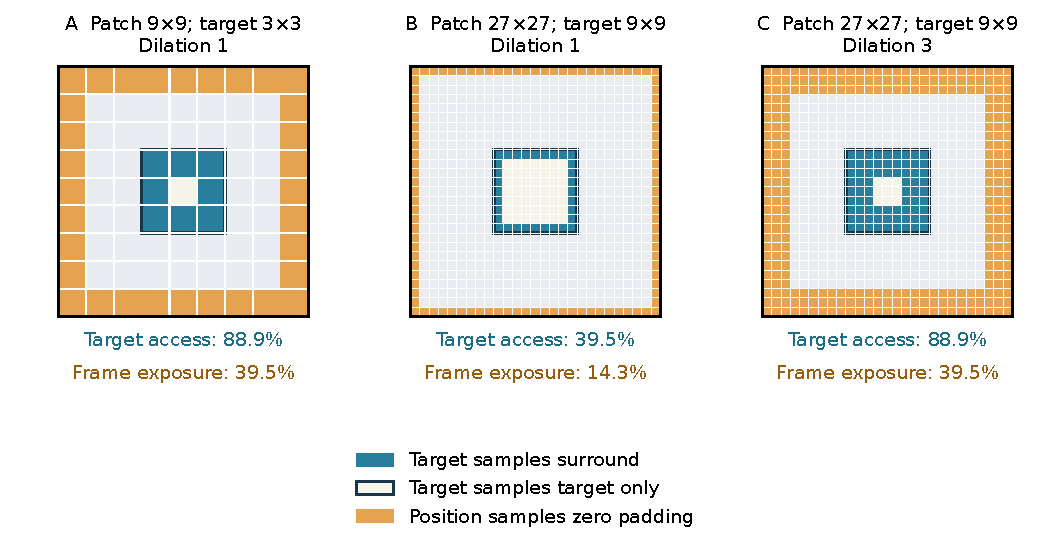
\includegraphics[width=\textwidth]{revision_figures/scale_geometry.pdf}
\caption{Spatial support in the three geometries. Colored target positions have sampled receptive fields reaching the surround; outer-frame shading marks whole-image positions exposed to zero padding. Dilation 3 uses a sparse $7\times7$ footprint. The target-access and padding fractions are derived from support, not fitted to the results. Recovery under dilation alone does not distinguish target boundaries from outer-frame contributions.}\label{fig:geometry}
\end{figure}

\subsection{Held-out scenes and informative reference cues}\label{sec:cues}
Natural-data classification reached training/validation/test accuracies of 93.4/95.0/65.8\% at 9 pixels and 94.1/95.4/65.4\% at 27 pixels. Test intervals were [61.3,70.6]\% and [61.0,70.2]\%. Twenty-nine of thirty seeds passed the validation gate at each size; every seed remained in the primary analysis. The generalization gap is therefore not explained by widespread failure to fit the training task. Synthetic-control test accuracy was 95.0\% and 93.3\%, underscoring dependence on the input source and partition. The historical high score cannot be equated with the current scene-disjoint score because its run-level protocol was not recovered.

The strongest reference-cue result concerns illuminant estimation. With an unknown surround, mean test $R^2$ was $-0.281$ and $-0.430$ at 9 and 27 pixels. With known neutral reflectance it rose to 0.968 and 0.971. RMSE fell from approximately 6750/7088 K to 817/673 K. Paired $R^2$ improvements were 1.249 [0.915,1.745] and 1.401 [0.991,1.952]. This result demonstrates substantial dependence on available information rather than unconditional inferiority of estimation.

In the natural-texture experiment, shuffled-minus-intact training changed base-readout test accuracy by $+0.0094$ [$-0.0055,0.0254$]. This does not establish an intact-context advantage or equivalence. Because the inserted target and crop are independently selected, it also does not test the value of ecological material adjacency.

Supplemental six-feature raw-cone decoding reached classification accuracies of 0.736 at both sizes, while temperature $R^2$ remained negative ($-0.595/-0.626$). Added noise did not clearly reduce category accuracy; illuminant-decoding $R^2$ improved but remained negative. These are separate supervised endpoints; comparing accuracy with $R^2$ does not establish an information-theoretic ranking.

\begin{figure}[p]\centering
\renewcommand{\baselinestretch}{1}\small
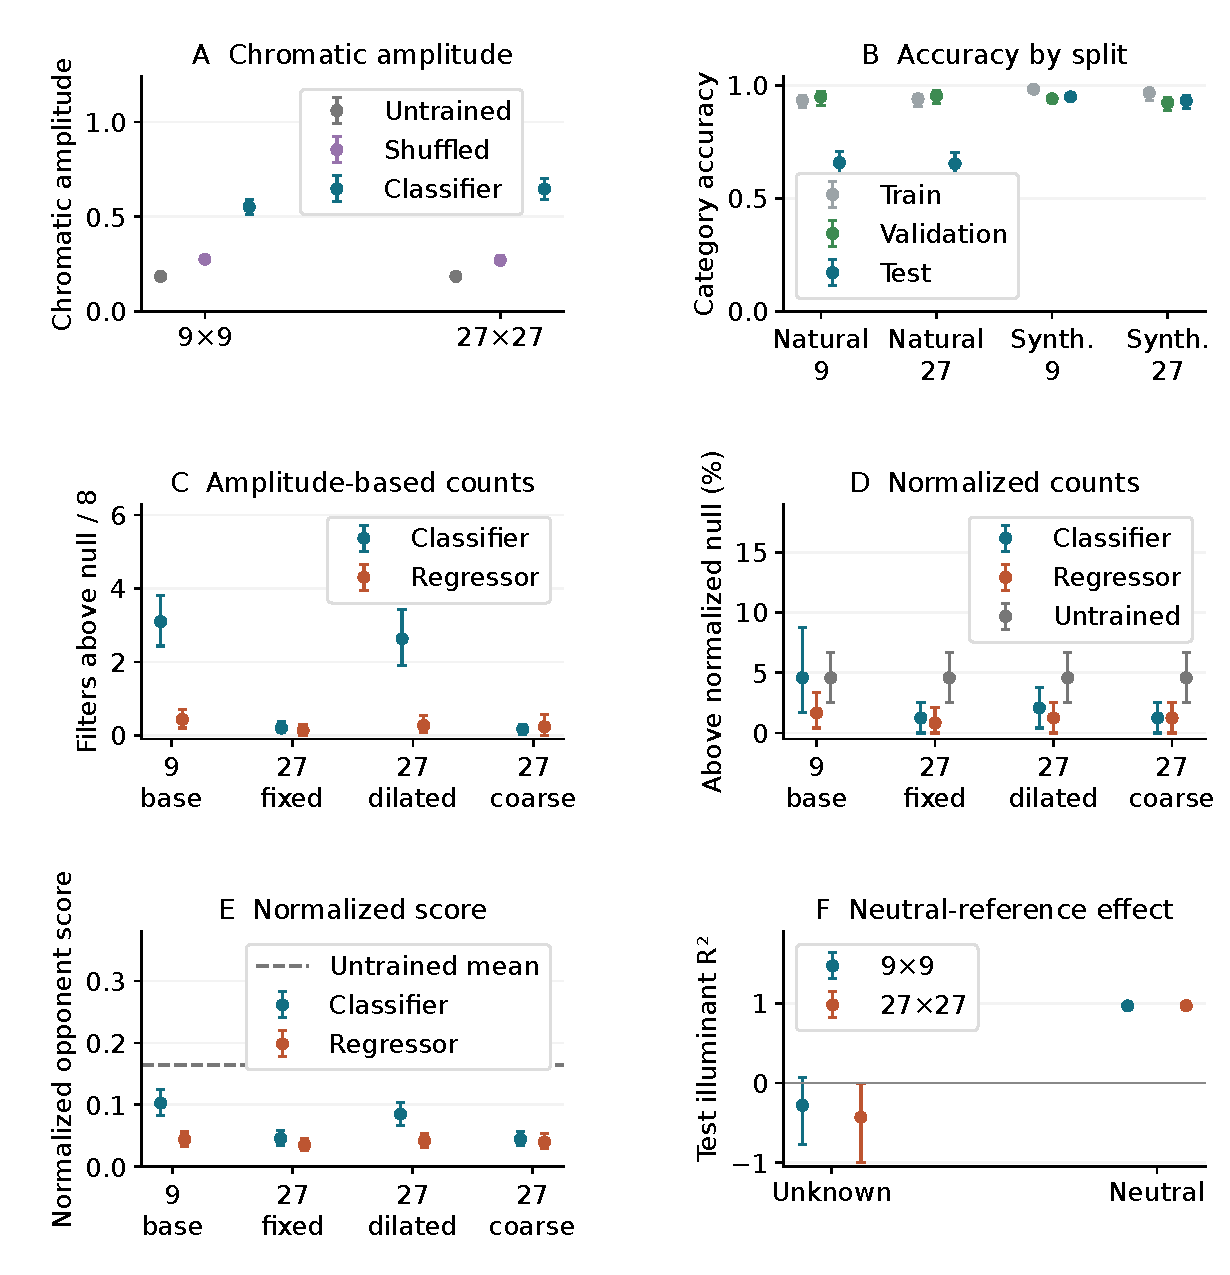
\includegraphics[width=\textwidth,height=0.73\textheight,keepaspectratio]{revision_figures/main_results.pdf}
\small
\caption{Learned color responses depend on endpoint and evaluation conditions. (A) Amplitude-based chromatic weights for initialized, shuffled-label, and category-trained networks. (B) Training, validation, and test category accuracy for natural and synthetic inputs. (C) Amplitude-based opponent counts for classifier and regressor across geometry controls. (D) Normalized above-null fractions. (E) Continuous normalized scores with initialization reference. (F) Illuminant-estimation $R^2$ with unknown and neutral-reference surrounds. Means and descriptive 95\% seed-bootstrap intervals use 30 seeds per condition and one fixed scene partition. The frozen primary normalized interaction is inconclusive; unlike metrics are not interchangeable.}\label{fig:main}
\end{figure}

\subsection{Local assimilation, global contrast, and limits of induction}\label{sec:illusions}
The unconstrained learned antagonism parameter was positive in all 30 seeds at each size: mean $b=0.401$ [0.362,0.436] at 9 and 0.271 [0.246,0.294] at 27. Calibrated global BY contrast occurred in all 27 valid learned-readout seeds at each size; three calibrations per size were undefined. Local target responses retained mean assimilation. In contrast, the base representation showed global BY assimilation of 0.0616, 0.0404, and 0.0653 for small, large-fixed, and large-dilated conditions. These signs concern the specified representations, not classifier labels or perceived appearance.

For $z=c-bs$, a surround perturbation produces $\Delta z=\Delta c-b\Delta s$. Local mixing and a globally antagonistic response can therefore coexist. A pooled scalar response does not demonstrate a spatially distributed change in distant target features. RG effects were less uniform than BY effects, further limiting a universal sign claim.

Distant watercolor features were exactly unchanged in all 25,212 finite measurements across the audited models and controls. All 18,909 finite distant Cornsweet differences were numerical zero (maximum absolute value $6.8\times10^{-21}$); 1,611 undefined calibrations were recorded separately. These large counts describe probe coverage, not independent samples. Near-contour and near-cusp responses can occur, including in controls, without establishing distant surface appearance.

Signed Mach responses predominantly indicated smoothing. The canonical BY overshoot index for the learned 9-pixel readout model was $-0.00243$ [$-0.00322,-0.00155$]. The initial workflow's unsigned score could not distinguish smoothing from overshoot, and its Cornsweet windows overlapped physically changed cusp pixels. Corrected endpoints therefore do not support a five-illusion unification (Fig.~\ref{fig:illusions}). These measurement limitations are distinct from the spatial-size effects; without historical raw outputs they do not identify the exact origin of every earlier figure value.

\begin{figure}[p]\centering
\renewcommand{\baselinestretch}{1}\small
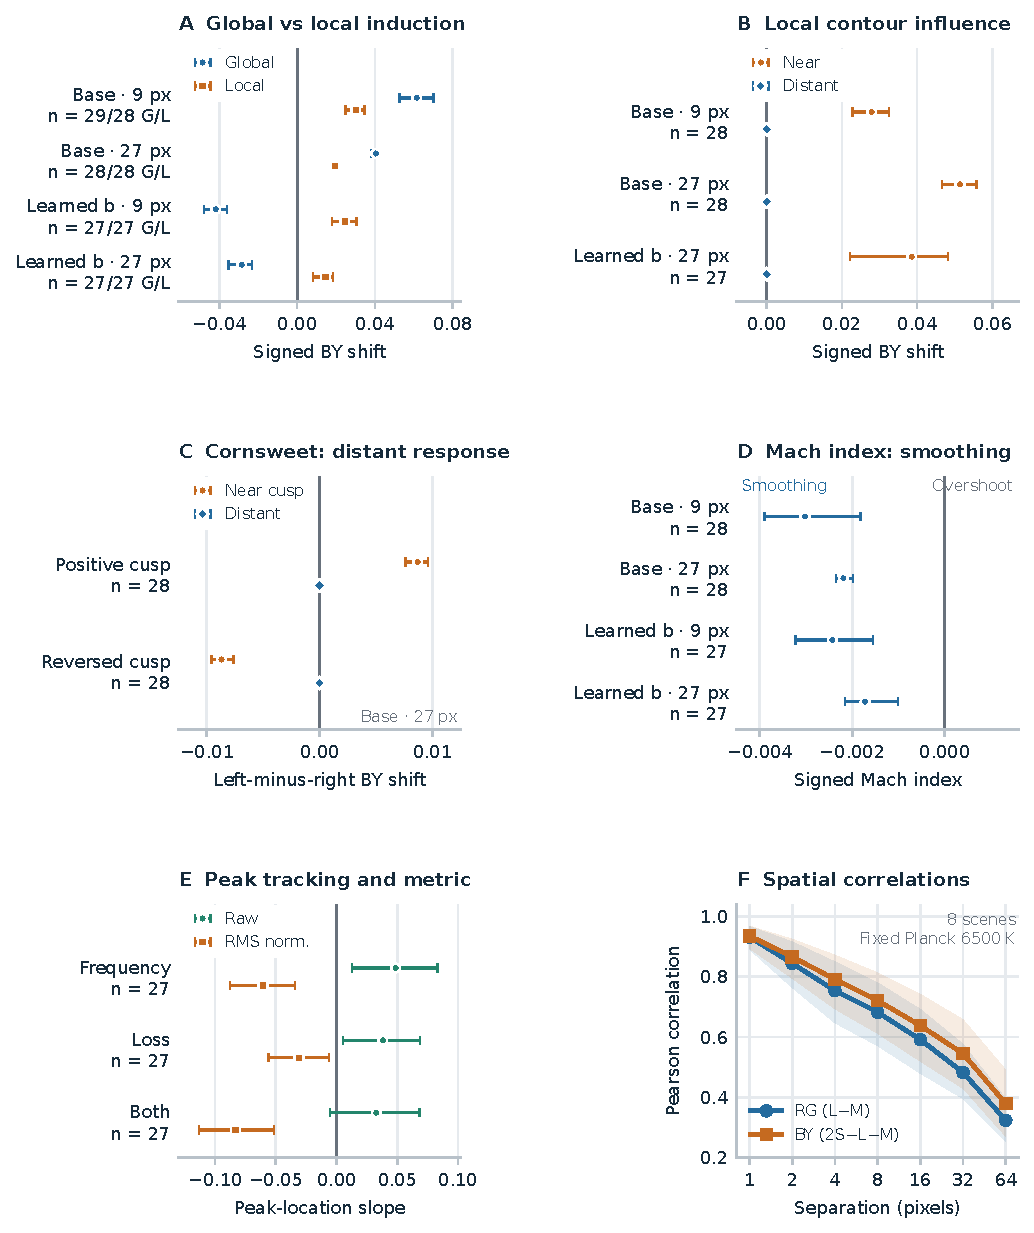
\includegraphics[width=\textwidth,height=0.73\textheight,keepaspectratio]{revision_figures/illusion_results.pdf}
\small
\caption{Signed induction and exploratory context measurements. (A) Global and local BY responses for base and learned-antagonism models; negative denotes calibrated contrast, positive assimilation. (B) Watercolor near-contour responses versus unchanged distant interiors. (C) Cornsweet near-cusp polarity reversal versus unchanged distant flanks. (D) Signed Mach index: positive would indicate canonical overshoot; displayed means have the smoothing sign. (E) Within-seed slopes relating imposed weighting locus to bounded-window sensitivity maxima, before and after RMS normalization. (F) Scene chromatic correlations versus pixel separation under a fixed generated 6500-K illuminant. Intervals are descriptive seed bootstraps (A--E) or scene bootstraps (F). Calibration counts are shown; E uses 27 complete non-flat seed blocks and F eight scenes. A nearby response or global output does not establish distant human filling-in.}\label{fig:illusions}
\end{figure}

\subsection{Architecture, optimization, utility, and environmental grounding}\label{sec:robustness}
Under the exploratory paired mean-sign-flip tests with Benjamini--Hochberg adjustment, the amplitude-based classification--estimation advantage survived across the twelve tested architectures at 9 pixels; none of these contrasts survived the corresponding adjustment at 27. For the normalized thresholded fraction, the frozen Holm procedure found no adjusted-significant objective contrast among the 24 architecture--size combinations (minimum adjusted $p=0.104$). Exploratory mean-sign-flip/BH analysis identified three positive small-pattern conditions and none at 27. Continuous normalized scores favored classification in ten of twelve small-pattern architectures and only the base architecture at 27. Counts, fractions, and testing procedures must therefore be distinguished.

Evolutionary and Adam optimization both supported category learning, with mean test accuracy 0.660/0.646 and 0.664/0.668, respectively, at 9/27 pixels in the matched-objective comparison. Their representations differed: the amplitude-based threshold classified 99.58\% of evolutionary filters as opponent, versus normalized fractions of 6.67/5.83\%. The evolutionary normalized score did not clearly increase over its matched initialization. This supports gradient-free task learning, not optimizer-invariant opponent organization; convergence and equivalence were not established.

Utility results also depended on normalization. Within-seed slopes of sensitivity-peak location against imposed locus were positive for raw sensitivity (frequency 0.0488, loss 0.0381, both 0.0328) but negative after RMS normalization ($-0.0606,-0.0309,-0.0832$). Each summary used 27 complete finite non-flat seed blocks. The physical BY probe range was approximately $[-0.05652,0.01022]$, narrower than the imposed loci $-0.2,0,0.2$; many maxima occurred at endpoints. Weighting also altered effective class balance. These results do not identify a global sensitivity optimum, a human discrimination threshold, or measured ecological benefit.

Mean nearest-cardinal distance in the specified log-cone convention was $18.42^\circ$ [$15.98,20.88$] for small-pattern classifiers versus $22.15^\circ$ [$20.76,23.43$] at initialization. However, classifier-minus-shuffled differences were inconclusive at both sizes: $-1.73^\circ$ [$-4.77,1.37$] and $0.39^\circ$ [$-2.66,3.47$]. Task-specific cardinal alignment is therefore not established. Across eight scenes, chromatic correlations decreased from 0.931/0.935 at one pixel to 0.323/0.379 at 64 pixels. These environmental observations agree qualitatively with spatially structured spectra, but do not identify the network's learning mechanism or a measured-daylight ensemble.

% All numerical results are post-production,
% exploratory saved-checkpoint diagnostics run on 24 November 2026.
% Source: scale_diagnostics/summary.json and identity_precision.json.
\subsection{Fixed-weight controls separate geometry from learned representations}
\label{sec:frozen_scale_controls}

To distinguish the immediate effect of geometry from differences acquired during training, we evaluated all 30 classifiers from each of the 9-pixel, 27-pixel fixed-kernel, and 27-pixel dilated-kernel conditions without updating their weights (Fig.~\ref{fig:diagnostics}). Each network was evaluated at patch widths of 9 and 27 pixels and dilations of 1 and 3, with a target occupying one third of the patch width. Noise-free simultaneous-induction probes used identical target and surround colors across geometries, on the RG and BY axes at both surround polarities and contrast magnitude 0.15. Raw signed projection numerators and separately calibrated local, global, and output-logit responses were retained; undefined calibrations remained undefined. These exploratory diagnostics were developed after the production results, with protocols specified before their execution. They are separate from the prespecified primary scale-by-objective endpoint.

With the 9-pixel-trained weights held fixed, the mean local blue--yellow target shift decreased from 0.03013 at width 9 and dilation 1 (95\% seed-bootstrap CI [0.02517, 0.03472]) to 0.00990 at width 27 and dilation 1 ([0.00800, 0.01166]). The paired decrease was $-0.02023$ [$-0.02306$, $-0.01716$], with 28 valid calibrations out of 30 seed blocks. Increasing dilation to 3 at width 27 restored the mean to 0.03013. Both groups trained at 27 pixels showed the same attenuation and restoration (Table~\ref{tab:frozen_scale}). The 27-pixel fixed-kernel weights give a higher mean local response on the shared 9-pixel probe (0.05423) than the 9-pixel-trained weights (0.03013), despite their lower amplitude-based opponent count. This descriptive comparison further separates calibrated functional response from a thresholded weight index. The controls demonstrate an immediate dependence on relative support without requiring differences in learned weights. They do not, by themselves, explain why separately trained networks acquired different weight-based scores.

\begin{table}[htbp]
\centering
\caption{Calibrated local blue--yellow target shifts for fixed saved weights. Positive values indicate assimilation. Columns specify the probe width and convolution dilation. Each row holds weights fixed; $n$ counts valid calibrations among 30 seed blocks and is the same across the three displayed columns. Full seed-bootstrap intervals and red--green, raw, global, and output-logit results are provided with the reproducibility data.}
\label{tab:frozen_scale}
\begin{tabular}{lrrrr}
\hline
Training condition & 9 / $d=1$ & 27 / $d=1$ & 27 / $d=3$ & $n$ \\
\hline
9-pixel, fixed kernel & 0.03013 & 0.00990 & 0.03013 & 28 \\
27-pixel, fixed kernel & 0.05423 & 0.01944 & 0.05423 & 28 \\
27-pixel, dilated kernel & 0.03314 & 0.01098 & 0.03314 & 27 \\
\hline
\end{tabular}
\end{table}

For this architecture, repeating each input pixel into a $3\times3$ block, tripling dilation, and copying weights preserves local feature maps up to repetition. Pointwise nonlinearities and the $1\times1$ convolution commute with repetition, and target/global means are preserved, giving identical representations and outputs in exact arithmetic. Tests on 32 random patches and 14 calibration/induction probes per seed exceeded the specified $10^{-6}$ float32 tolerances in some arrays (maximum logit difference $6.48\times10^{-5}$). A separately specified float64 follow-up passed $10^{-12}$ tolerances for all 30 networks (maximum difference below $1.8\times10^{-14}$), supporting an accumulation-precision explanation. Both outcomes are retained in the release. Independently sampled 27-pixel noise and non-repeated Cornsweet, Mach, and watercolor profiles do not satisfy this exact-input identity.

We also replaced zero padding with replicate or reflect padding after training, using the same test trials for all 90 classifiers. Replicate padding changed 2.82\%, 1.10\%, and 3.37\% of predictions for the 9-pixel, 27-pixel fixed, and 27-pixel dilated groups, respectively. Mean accuracy changes were $+0.500$ percentage points [95\% CI $-0.197$, $+1.193$], $+0.083$ [$-0.283$, $+0.480$], and $+0.360$ [$-0.413$, $+1.097$], using all 30 seeds per group. Reflect padding gave similar results. Local target BY shifts were exactly unchanged, consistent with target receptive fields not reaching the frame, while global representations changed. Thirty intact-context center-only classifiers supplied a negative control: neither padding replacement changed any predicted label or accuracy; logit differences were limited to float32 roundoff. These post-training interventions distinguish local induction from frame-sensitive global readouts. Their effects during learning remain unresolved.

\begin{figure}[p]\centering
\renewcommand{\baselinestretch}{1}\small
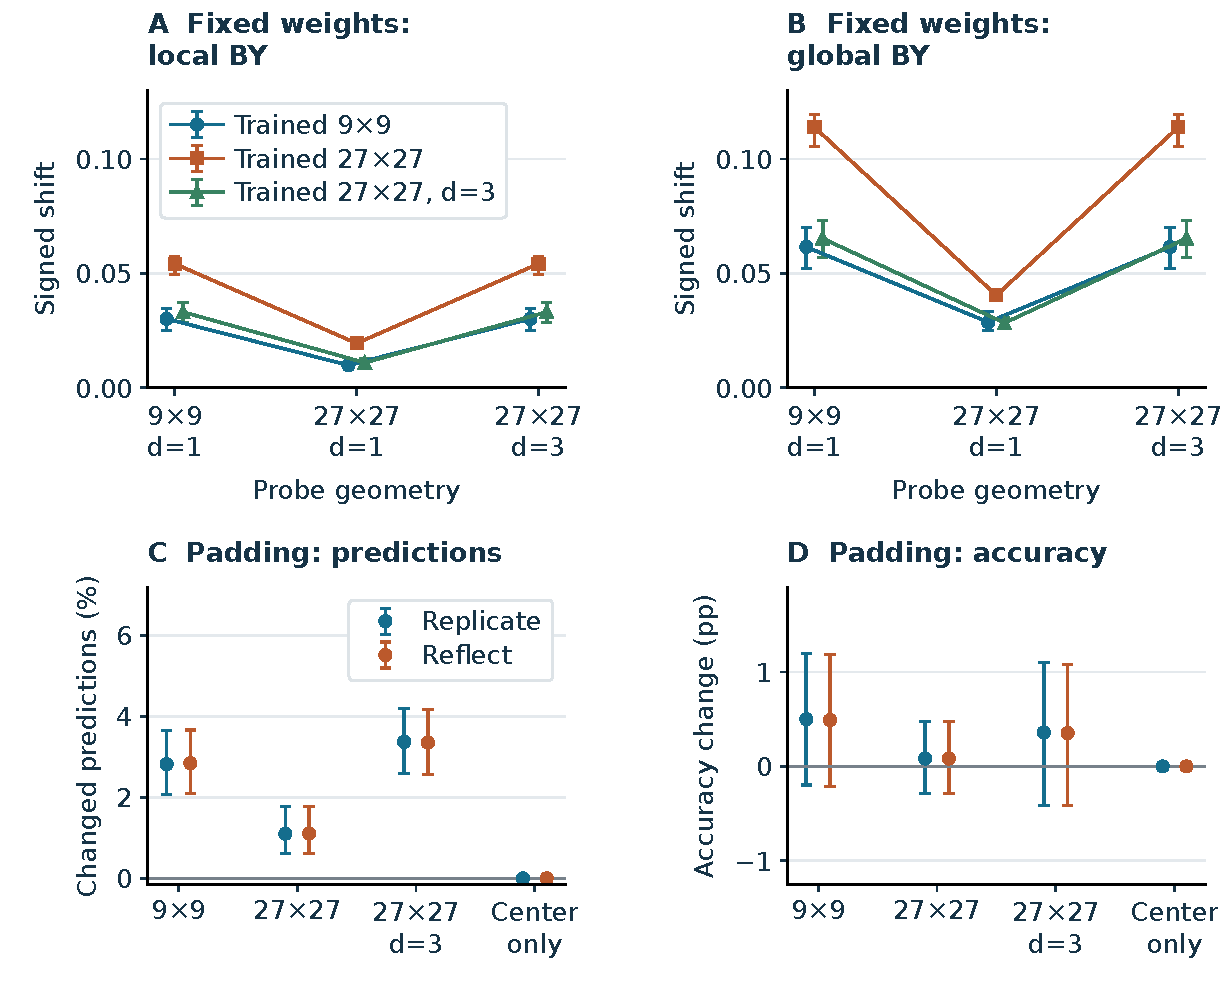
\includegraphics[width=\textwidth,height=0.73\textheight,keepaspectratio]{revision_figures/fixed_weight_controls.pdf}
\caption{Exploratory fixed-weight controls. (A,B) Local and global BY induction across probe width/dilation combinations, with a separate curve for each training geometry. Positive denotes assimilation and negative contrast. Within each curve the weights are unchanged; undefined calibrations are excluded. For training at 9 pixels, 27 pixels with fixed support, and 27 pixels with dilation, valid counts are 28/28/27 locally and 29/28/27 globally. (C,D) Prediction changes and paired accuracy differences when zero padding is replaced after training by replicate or reflect padding. These panels use all 30 seeds per condition; the center-only control uses 27-pixel patches. Intervals are descriptive 95\% seed bootstraps. Local target responses remain unchanged by padding replacement, while some global predictions change.}\label{fig:diagnostics}
\end{figure}


\section{Discussion}\label{sec:discussion}
\subsection{What the two spatial sizes reveal}
Retaining both geometries is more informative than replacing the original condition with a larger raster. The small target is dominated by locations having access to a boundary; the large fixed-kernel target contains more locally isolated interior. Dilation restores access and accompanies recovery of local induction and several weight-based measurements. The model nevertheless retains global context through its pooled readout, so similar accuracy can coexist with different local organization. This is a plausible allocation of computation, not proof that the network no longer uses context.

The physiological analogy concerns chromatic integration and differentiation. V1 experiments distinguish responses to extended regions from responses to chromatic spatial patterns \citep{johnson2008orientation,conway2006spatiotemporal}. Functional double-opponent fields can be nonconcentric and do not require perfect spatial balance \citep{de2021spatial,de2022coding}. These findings support direct functional testing and caution against identifying either computational index with neuronal prevalence. They do not imply that increasing image size must reduce biological opponency or prescribe the weights learned by an optimizer.

Indeed, enlarging grating apertures can strengthen relative chromatic responsiveness and band-pass tuning \citep{solomon2004surrounds}. That manipulation adds surround stimulation while holding carrier frequency fixed; our manipulation separates a target's boundaries relative to a fixed kernel. Human size effects also depend on chromatic configuration rather than a single universal direction \citep{canham2021size,kanematsu2022size}. Temporal-frequency-dependent physiological tuning and depth-dependent network tuning provide further evidence for assay dependence, without mapping our static patches onto particular cortical stages \citep{songlin2026chromatic}.

The current scale account is therefore conditional. It is strongest as a support constraint on local responses and as a hypothesis about how training uses boundary and surface signals. Zero-padding exposure, noise covariance, and natural-crop extent must be separated before assigning a unique causal mechanism. Acute responses of fixed weights to changed stimuli and the weights learned by separate networks answer different questions.

\subsection{Task, reference information, and related models}
Task-dependent color categories and opponency have precedents in object-recognition and bottleneck studies \citep{devries2022categorization,harris2021opponency}. CLIP-like semantic attribution and segmentation tolerance extend the range of relevant behaviors, but those endpoints differ from local induction or physiological cell classification \citep{arias2024clip,hernandezcamara2024alignment}. Our contribution is a controlled comparison across objectives, spatial supports, and measurements, with negative controls and an explicitly inconclusive primary result.

The neutral-reference rescue places the estimation comparison in a broader context. Human constancy can use multiple scene cues, and removing or contradicting contextual information changes model performance \citep{kraft1999constancy,flachot2022deep,heidari2026human}. Illuminant-prediction networks can themselves learn opponent-like filters, while temporal self-supervision can support constancy \citep{gao2026illuminant,ernst2024selfsup}. Thus classification is one route to useful color representations, rather than an exclusive origin. The relative difficulty of our two tasks depends on the information supplied by the rendering model and surrounding surfaces.

\subsection{Why induction agreement must be measured separately}
Prior CNN work already showed that stimulus size, kernels, dilation, and training task affect illusion-like responses \citep{gomezvilla2019deceived}. Its quantitative follow-up exposed departures from human signs despite opponent channels \citep{gomezvilla2020color}. Our local/global distinction is consistent with that separation between representation and appearance.

Human watercolor assimilation can weaken as the enclosed region grows yet persist across distant interiors \citep{devinck2006watercolor}. Open contours can also support watercolor \citep{cohenduwek2019filling}. Our unchanged distant local features identify a limitation of the tested representation, whereas pooled contrast establishes a different computation. Edge integration and multiscale filtering offer candidate additions \citep{rudd2014edge,otazu2010chrom}; neither literal diffusion nor a unique cortical site follows from the present data. Similarly, approximate scale invariance of human Mach-band visibility constrains an explanation based solely on larger patterns \citep{wallis2012mach}. Correct sign and physically matched regions are necessary before claiming perceptual agreement.

\subsection{Limitations and discriminating tests}\label{sec:limitations}
The study has one eight-scene partition, approximate cone sensitivities, generated Planck illuminants, endpoint duplication at 400 nm, and retained clipping conventions. The category definition is based on two spectral quartiles rather than natural object identities. Our architecture has one local spatial support followed by global pooling and lacks validated temporal adaptation or perceptual calibration. Functional neuronal assays, direct human/model matching, and additional scene partitions are needed for stronger biological and generalization claims.

The normalized primary interaction remains inconclusive. Descriptive recovery in other endpoints cannot replace it. Likewise, the scene-disjoint accuracy gap, readout-dependent signs, normalization-sensitive utility results, and historical measurement limitations should not all be attributed to scale. No calibrated Dress experiment was recovered, so that phenomenon is outside the empirical claims of this revision. The analytic ecological proxies do not establish measured ecological payoffs.

Further tests should independently vary target width and receptive-field support, compare matched noise covariance and outer-padding conventions during training, and measure signed cone/spatial responses before and after controlled perturbations of opponent components. A functional difference need not be behaviorally necessary if the readout is redundant. Human comparisons require a common matching or nulling endpoint and one declared visual-angle mapping, rather than adjusting scale separately for each illusion. New confirmatory contrasts should be specified before collection, without changing the interpretation of the frozen primary result.

\section{Reproducibility and availability}\label{sec:reproducibility}
The release at \url{https://github.com/rostami-m/color_evolution}, tag \texttt{visionresearch-revision-20261124}, provides the active experiment implementation, dependency specification, explicit data preparation, frozen condition metadata, compact result tables, and scripts regenerating the manuscript figures. Instructions distinguish regenerating figures from the published summaries from retraining the complete study from source data. Natural-scene files and checkpoints are not silently substituted by synthetic data. Full training is computationally more expensive than figure regeneration, and numerical backend/version differences can change fitted weights.

Independent integrity checks found all 6,870 expected records and checkpoints, the prescribed training budgets, and finite required primary metrics and performance values; all 43 frozen scientific source hashes matched. Fourteen representative checkpoints were reconstructed on CPU and exactly reproduced their saved filter metrics and test summaries. A separate release-compatibility check compared 18 production checkpoints across classification, regression, readout, and optimization conditions: test inputs, predictions, metrics, and signed probes matched exactly between the frozen and portable implementations. All 2,431 production configuration dictionaries also matched. These checks support record/evaluation consistency, not the validity of every modeling assumption or equivalence of training backends. The code--manuscript audit and the release's tests document the relationship between the production snapshot and the portable implementation. The primary/secondary distinctions, undefined calibrations, seed-level results, and environmental assumptions are retained for inspection.

\section{Conclusion}
In this constrained color-learning model, task objective, relative spatial support, contextual reference information, and readout jointly shape measured color responses. Enlarging the target with fixed support attenuates local induction and several weight-based measures, while dilation restores much of them. These observations coexist with an inconclusive normalized primary interaction, cue-dependent estimation, and failures of distant or correctly signed illusion responses. The small and large experiments therefore delimit the conditions under which a learned representation resembles selected aspects of color processing, rather than establishing a universal account of human color appearance.

\section*{CRediT authorship contribution statement}
\textbf{Mohammad Rostami:} Conceptualization, Methodology, Software, Formal analysis, Investigation, Data curation, Visualization, Writing -- original draft, Writing -- review \& editing.
\section*{Declaration of competing interest}
The author declares no competing interests.
\section*{Funding}
This research received no specific grant from funding agencies in the public, commercial, or not-for-profit sectors.
\section*{Declaration of generative AI and AI-assisted technologies in the manuscript preparation process}
Claude was used for LaTeX-formatting assistance during preparation of the initial manuscript. OpenAI Codex was used during revision to assist with literature retrieval, software implementation and checks, analysis, and drafting. The author retains responsibility for the scientific interpretation, verification of sources and results, and final manuscript.
\section*{Acknowledgements}
The author thanks the investigators and maintainers who made the Foster natural-scene hyperspectral data publicly available.
\section*{Data availability}
The source Foster scenes are publicly distributed by the original investigators. The code release documents the source links, checksums, preprocessing, scene partition, and explicit synthetic controls. Compact derived results and figure-generation code accompany the repository. No redistribution right for the source hyperspectral files is assumed.
\bibliographystyle{elsarticle-harv}
\bibliography{references}
\end{document}
